The intuition behind NBFNet, is that many of the traditional link-prediction heuristics such as Katz-Index, Personalized PageRank~\cite{Page1998PageRank} or Graph Distance can be generalized into a
\textit{multiplication} and a \textit{summation} step.

\begin{figure}[h] % [h] attempts to place figure here, other options like [t]op, [b]ottom
    \centering % Centers the figure horizontally
    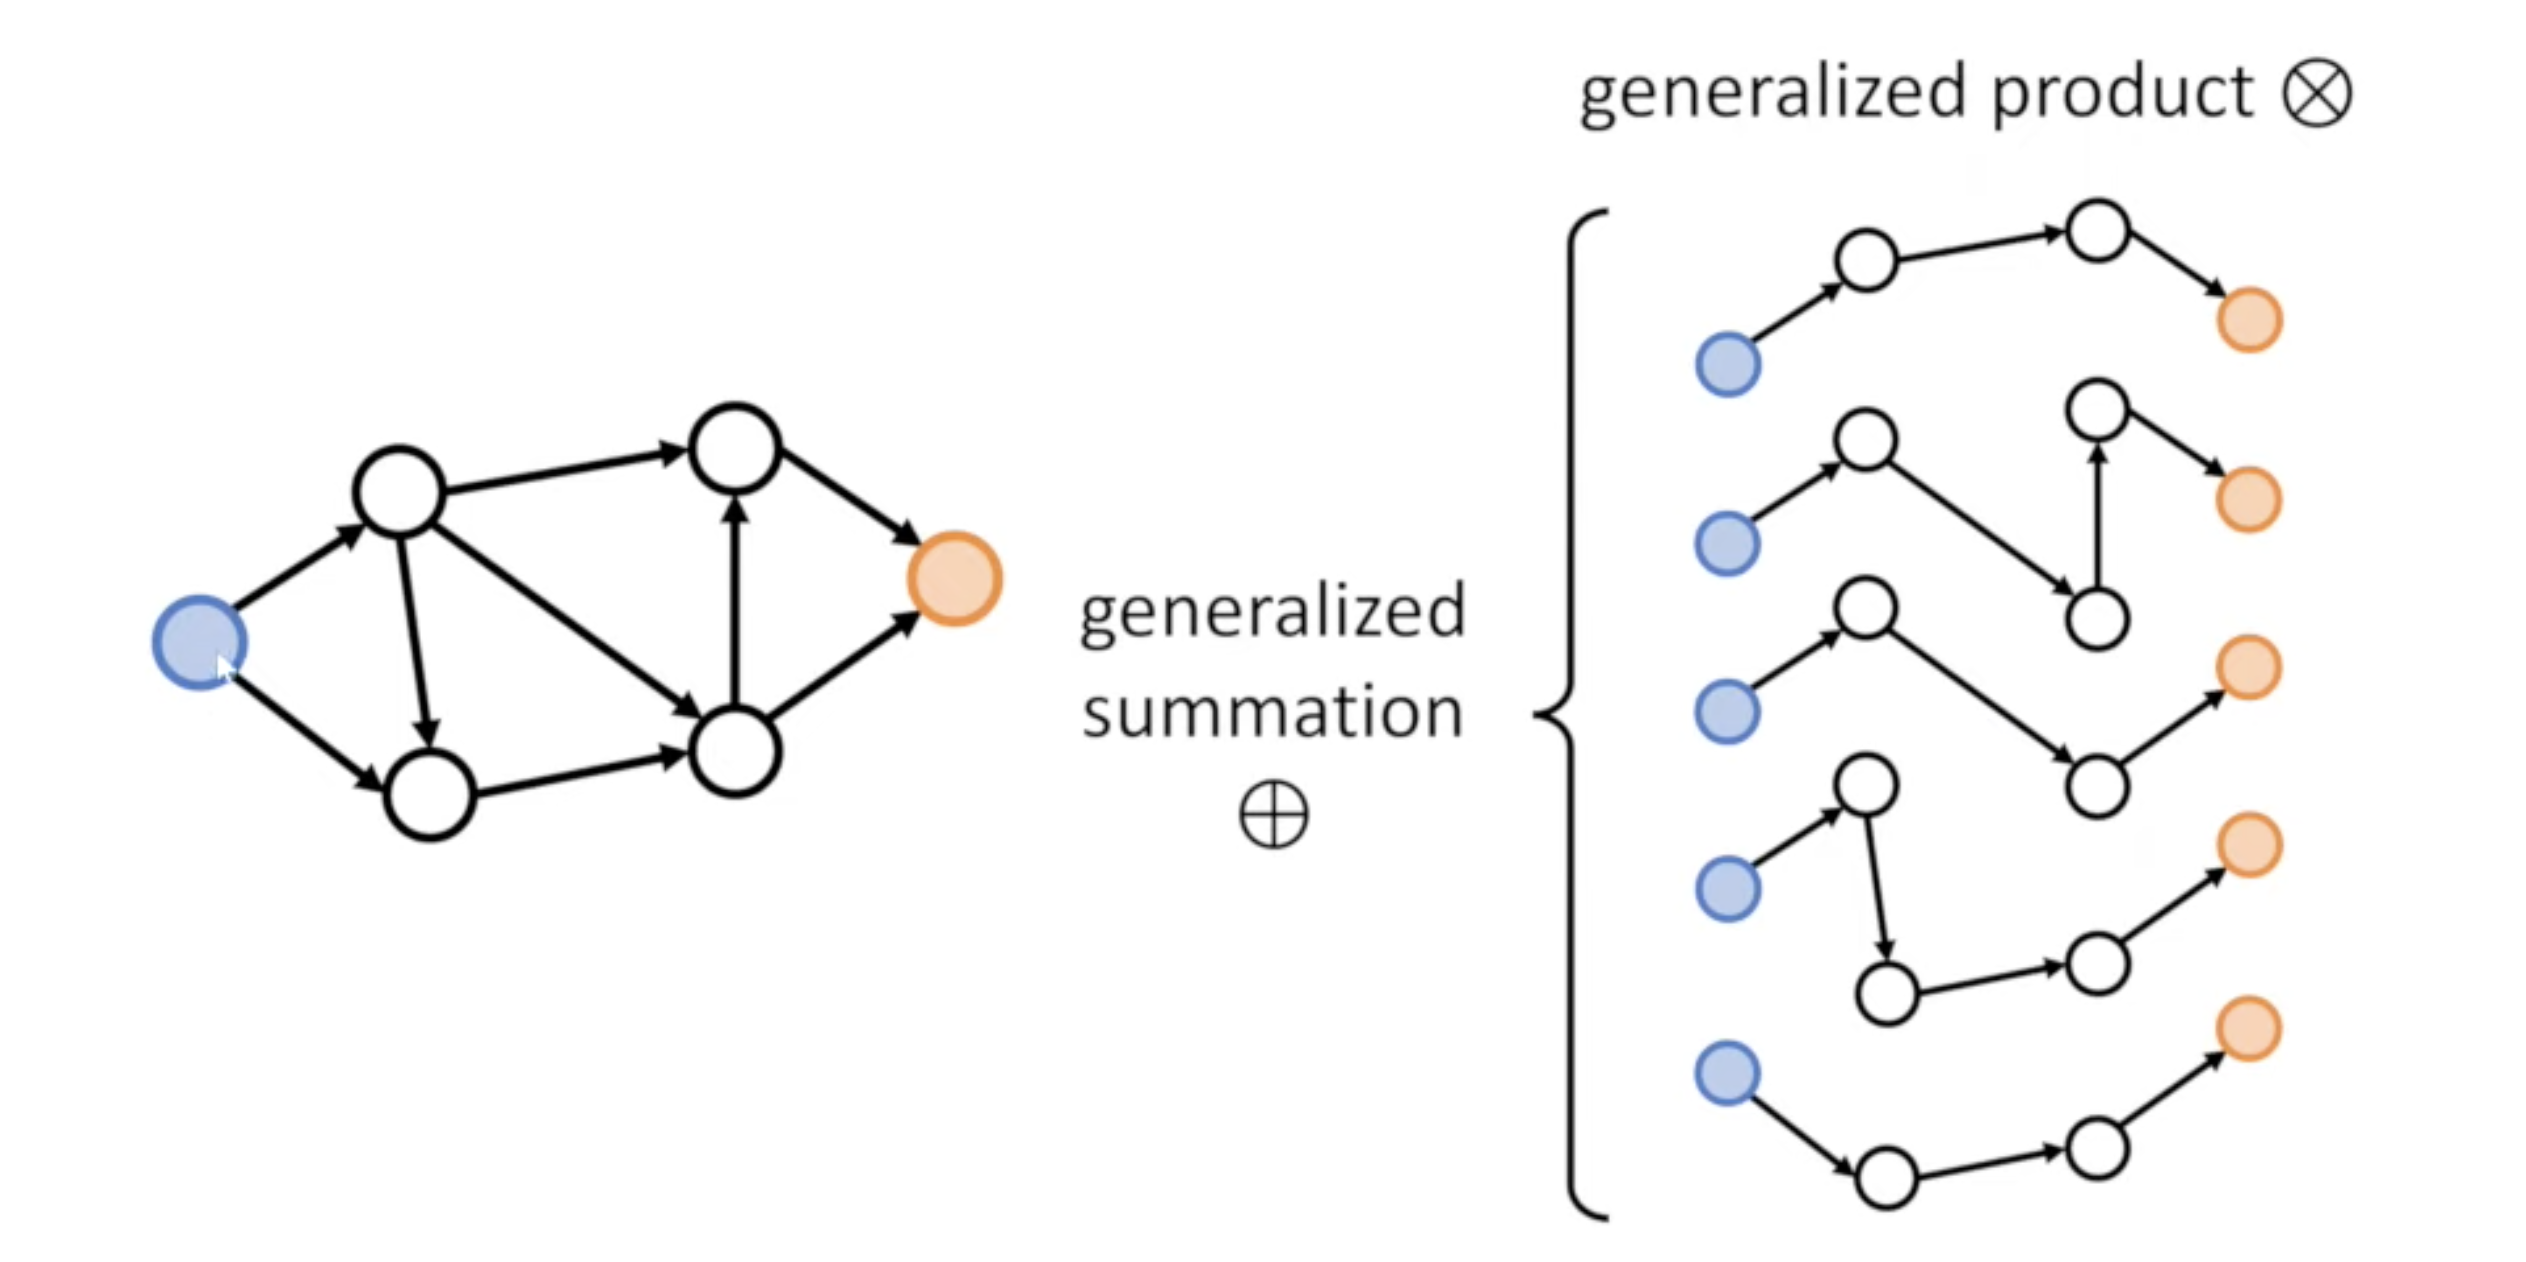
\includegraphics[width=0.8\linewidth]{figures/nbfnet-trad} % Include the image with desired width
    \caption{Generalized Graph Heuristic ~\cite{NBfnetPres}} % Add a caption
    \label{fig:nbfnet-trad} % Assign a label for referencing the figure in text
\end{figure}.

Path Formulation. Link prediction is aimed at predicting the existence of a query relation q between a head entity u and a tail entity v. From a representation learning perspective, this requires to learn a pair representation hq(u,v), which captures the local subgraph structure between u and v w.r.t. the query relation q. In traditional methods, such a local structure is encoded by counting different types of random walks from u to v [35, 15]. Inspired by this construction, we formulate the pair representation as a generalized sum of path representations between u and v with a commutative summation operator ⊕. Each path representation hq (P ) is defined as a generalized product of the edge representations in the path with the multiplication operator 